%%%%%%%%%%%%%%%%%%%%%%%%%%%%%%%%%%%%%%%%%%%%%%%%%%%%%%%%%%%%%%%%%%%
%TO AVOID FORMATTING ISSUES, COMPILE THIS ONLY AT WWW.OVERLEAF.COM%
%%%%%%%%%%%%%%%%%%%%%%%%%%%%%%%%%%%%%%%%%%%%%%%%%%%%%%%%%%%%%%%%%%%
%%%%%%%%%%%%%%%%%%%%%%%%%%%%%%%%%%%%%%%%%%%%%%%%%%%%%%%%%%%%%%%%%%%
\documentclass[a4paper,12pt]{article}
\usepackage{graphicx}
%To use this font, you need XeTex or LuaTex, prefer openleaf
\newenvironment{codeblock}{\fontfamily{ccr}\selectfont}{\par}

\title{
	\normalfont \normalsize 
	\textsc{Pimpri Chinchwad College of Engineering \\ 
		Computer Laboratory - IV} \\
	[10pt]   
	\rule{\linewidth}{0.5pt} \\[6pt] 
	\huge Assignment no - B3 \\
	\rule{\linewidth}{2pt}  \\[10pt]
}
\author{}
\date{\normalsize}


\begin{document}
	\maketitle

\textbf{AIM: } A mobile application needs to be designed for using a Calculator (+, - ,*, /, Sin, Cos, sq-root) with Memory Save/Recall using Extended precision floating point number format. Give the Required modeling,Design and Positive-Negative test cases.\\\\


\noindent \textbf{OBJECTIVE:}
\begin{itemize}
\item To study the creation of a calculator application using java and android technology.
\item To study memory save/recall operations using extended floating point numbers. 
\end{itemize}
\noindent \textbf{UML diagrams:}\\
\begin{itemize}
\item \textbf{Class diagram:}
\begin{figure}[h!]
		\centering
		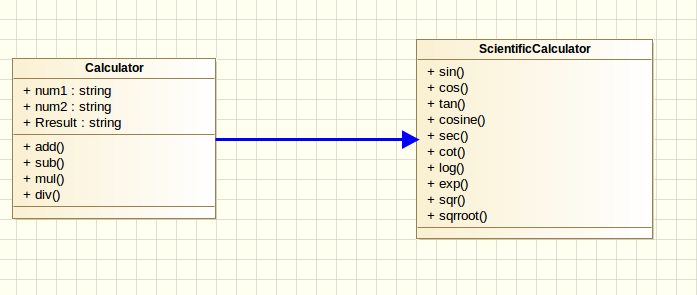
\includegraphics[scale=0.5]{calculator.png}
	\end{figure}



\newpage
\item \textbf{Use Case diagram :}
\begin{figure}[h!]
		\centering
		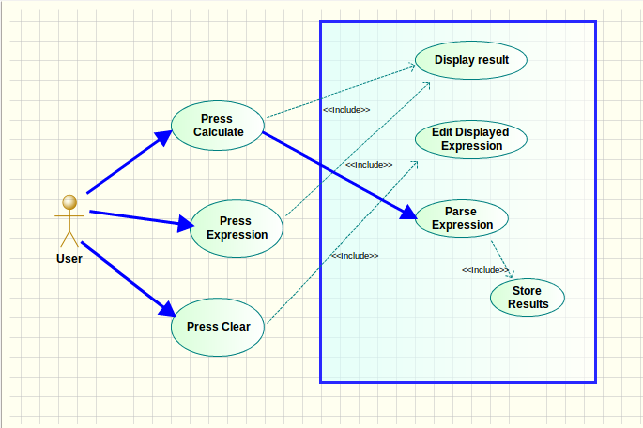
\includegraphics[scale=0.5]{usecase.png}
	\end{figure}

\item \textbf{Sequence diagram :}
\begin{figure}[h!]
		\centering
		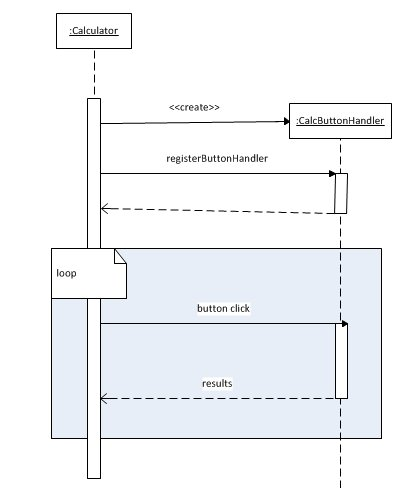
\includegraphics[scale=0.5]{calcseq.jpg}
	\end{figure}

\end{itemize}

\bigskip\bigskip
\bigskip\bigskip
\noindent \textbf{MATHEMATICAL MODEL :}\\[0.5cm]
S=\{s,e,X,Y,Fme,DD,NDD\}\\


\textbf{s=Initial State}\\
No input is provided to the textbox when the app is opened.

\textbf{e=End State}\\

Memory save/recall operations are performed and the result is shown in an appropriate form in the app. All the functions or the operations that the user needs are available to the user and the user must be able to perform all the operations.
\\

\textbf{X=Input given}\\

The input given to the app are numbers on which certain operations are performed or a particular expression that needs to be solved.
\\

\textbf{Y=Output obtained}\\

  The output of the app will be obtained when we solve the expression. It will give correct output on correct input and it will give wrong output on wrong input of data.
 \\

\textbf{Fme=Function/Algorithm}\\

The algorithm consists of functions like sine, cosine,and tan and memory save/recall operations. As the calculator performs basic as well as scientific functions, it will contain all the required functions.
\\

\textbf{DD=Deterministic data}
There is no deterministic data in the application.
\\

\textbf{NDD=Non-deterministic data}
The output will be dependent upon what input the user provides. 
\\

\noindent \textbf{THEORY:}	\\
\begin{itemize}
\item \textbf{Mobile App:}
A mobile app is a computer program designed to run on mobile devices such as smartphones and tablet computers. Most such devices are sold with several apps bundled as pre-installed software, such as a web browser, email client, calendar, mapping program, and an app for buying music or other media or more apps. 
\end{itemize}
\begin{itemize}
\item \textbf{Memory Save/Recall operations}
    Description of each button:

    MC = Clears the memory

    MR = Recall value in memory

    MS = Save value into memory

    M+ = Adds the currently displayed number on your calculator to the  number in memory

    M = Subtracts the currently displayed number from the number in memory
\end{itemize}
\begin{itemize}
\item \textbf{Extended Floating point numbers:}\\
Two classes of extended floating-point formats: single extended and double extended.

The standard does not prescribe the exact precision and size of these formats, but it does specify the minimum precision and size. For example, an IEEE double extended format must have a significand precision of at least 64 bits and occupy at least 79 bits overall.

Extended precision refers to floating point number formats that provide greater precision and more exponent range than the basic floating point formats.Extended precision formats support a basic format by minimizing roundoff and overflow errors in intermediate values of expressions on the base format. In contrast to extended precision, arbitrary-precision arithmetic refers to implementations of much larger numeric types (with a storage count that usually is not a power of two) using special software (or, rarely, hardware).
\end{itemize}
\begin{itemize}
\item \textbf{Android :}\\
Android is the name of the mobile operating system owned by American company; Google. It most commonly comes installed on a variety of smartphones and tablets from a host of manufacturers offering users access to Google�s own services like Search, YouTube, Maps, Gmail and more.

This means you can easily look for information on the web, watch videos, search for directions and write emails on your phone, just as you would on your computer, but there�s more to Android than these simple examples.

Android phones are highly customisable and as such can be altered to suit your tastes and needs; with wallpapers, themes and launchers which completely change the look of your device's interface. You can download applications to do all sorts of things like check your Facebook and Twitter feeds, manage your bank account, order pizza and play games. You can plan events on from your phone's calendar and see them on your computer or browse websites on your desktop and pick them up on your phone.

There are hundreds of thousands of apps and games available to download from the Google Play store (formerly the Android Market). There are camera apps that allow you to take pictures with artistic effects and music players which allow you to stream music from the web or create playlists. You can customise the appearance of your Android handset with a number of wallpapers based on pictures you�ve taken yourself or downloaded from the internet too.
\end{itemize}


\noindent \textbf{TESTING:}
\begin{itemize}
\item \textbf{Positive Testing:}\\
Positive Testing is testing process where the system validated against the valid input data. In this testing tester always check for only valid set of values and check if a application behaves as expected with its expected inputs. The main intention of this testing is to check whether software application not showing error when not supposed to and showing error when supposed to.

The system will show the appropriate output when it is tested against correct mathematical values. For example, for trigonometric functions, the system will show appropriate output in floating point numbers. Also for basic mathematical operations like addition, subtraction, it will show appropriate output.

\item \textbf{Negative Testing:}\\
Negative Testing is testing process where the system validated against the invalid input data. A negative test checks if a application behaves as expected with its negative inputs. The main intention of this testing is to check whether software application not showing error when supposed to and showing error when not supposed to.

While performing the negative testing, the system will show incorrect output while performing the basic arithmetic operations if the user enters only a single number and performs addition without entering the second number. The system will give an error when the user attempts a divide by zero operation.
\end{itemize}

\begin{itemize}
\newpage
\item \textbf{Test cases using black box testing:}
\begin{enumerate}
\item Test case: Part 1
\end{enumerate}
\begin{figure}[h!]
		\centering
		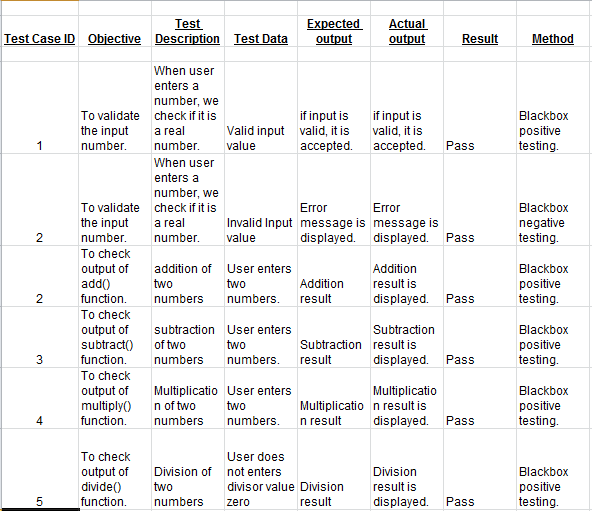
\includegraphics[scale=0.5]{testcase1.png}
	\end{figure}
    
\begin{enumerate}
\item Test case: Part 2
\end{enumerate}

\begin{figure}[h!]
		\centering
		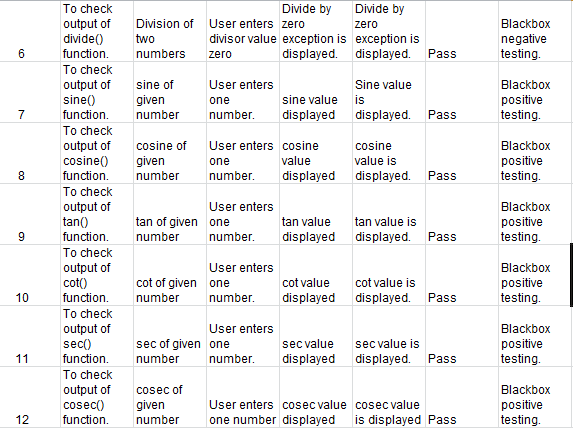
\includegraphics[scale=0.5]{testcase2.png}
	\end{figure}
\end{itemize}
\bigskip
\bigskip
\bigskip
\bigskip
\bigskip
\bigskip
\bigskip
\bigskip
\bigskip
\bigskip
\bigskip
\bigskip
\bigskip
\bigskip
\bigskip
\bigskip
\bigskip
\bigskip
\bigskip
\bigskip
\bigskip
\bigskip
\bigskip
\bigskip
\bigskip

\noindent \textbf{CONCLUSION:- }	\\
We have studied and implemented an android application for the development of calculator app in android using java programming language and using extended floating point and memory recall operations.

\begin{center}
\begin{tabular}
{|c|c|c|c|c|}\hline
{\bf Roll No.}		&{\bf Name of Student}	&{\bf Date of Performance}  				&{\bf Date of Submission}	&{\bf Sign.}  \\    \hline
{302}	&	{Abhinav Bakshi}& 	{15/02/16}	&  {29/02/16} \\ \hline
\end{tabular}\\ 
\end{center}


\begin{figure}[htb!]
	\centering
	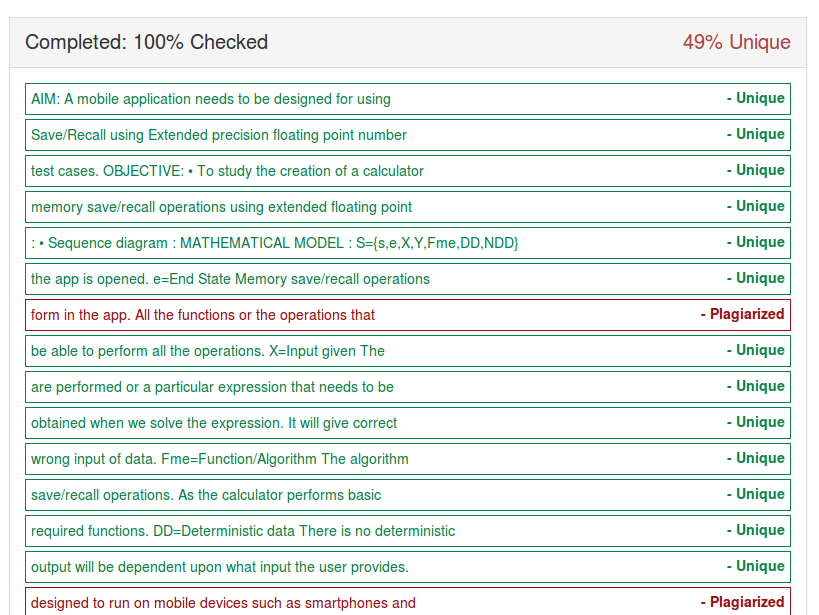
\includegraphics[scale = 0.80]{Trig.png}
	\caption{Plagiarism Report }
	\label{Plagiarism Report}
\end{figure}


\end{document}



 